
\section{XeonPhi}

\subsection{Introducci\'on}

La arquitectura Xeon Phi es la culminaci\'on de un trabajo iniciado por Intel en 2004, previendo
la necesidad de paralelismo masivo para aplicaciones futuras. Saliendo al mercado al final de 2012,
con el prop\'osito de competir en computo intensivo con NVIDIA CUDA, ha ganado gran tracci\'on dentro
de HPC a pesar de ser joven. Por ejemplo, ha sido fuertemente utilizada en la supercomputadora Tianhe-2 
de la Universidad de Sun Yat-Sen en China, listada en Top 500 como la supercomputadora m\'as r\'apida del
mundo en Junio 2013, Noviembre 2013 y Junio 2014~\cite{Top500XeonPhiJune2013},~\cite{Top500XeonPhiNov2013},~\cite{Top500XeonPhiJune2014}. Los 16000 nodos de esta supercomputadora contienen, adem\'as de dos Ivy Bridge Xeon, 3 coprocesadores
XeonPhi, dando un total te\'orico de 54.9 petaflops.

\subsection{Dise\~no de los procesadores}

\subsubsection{Microarquitectura general} 

En la concepci\'on del Xeon Phi se tuvieron en cuenta diversos factores, entre los cuales
se incluye el consumo energ\'etico. Uno de los objetivos fue disminuir la relaci\'on de
poder de c\'omputo por watt de los procesadores de Xeon de la \'epoca, manteniendo una entorno
de desarrollo de prop\'osito general como el de esta arquitectura. 
Si bien el consumo no se ve\'ia impactado por el set de instrucciones, 
si se busc\'o eliminar diversas partes del procesador:, intentando mantener 
caracter\'isticas que sirvieran al tipo de aplicaci\'on a la que se estaba 
apuntando (programas altamente paralelos a nivel de datos y tareas)~\cite{BookXeonPhi}.

La microarquitectura de este coprocesador se basa fuertemente en muchos procesadores sim\'etricos (SMP), al menos 50, lo
cual justifica su nombre MIC (\textit{Many Integrated Core}). El objetivo, adem\'as de proveer un dise\~no
capaz de escalar a las necesidades de aplicaciones fuertemente paralelas, es permitir que las mismas puedan
ser desarrolladas con herramientas lo m\'as similar posibles a las existentes: cada procesador esta basado
en el dise\~no del Intel Pentium, con una ISA (\textit{Instruction Set Architecture}) muy similar a la de este.
Los agregados a la arquitectura son soporte para direccionamiento a 64 bits y nuevas instrucciones de vectorizaci\'on.

Los procesadores tienen un \textit{clock rate} de 1.0 GHz aproximadamente, haciendolos bastante lentos frente
a otros procesadores de Intel. Por ejemplo, los procesadores de un Intel Xeon CPU E5-2620 tienen un \textit{clock rate}
de 2.10 GHz, aproximadamente el doble.

Un esquema de la arquitectura de cada procesador puede verse en la figura~\ref{fig:xeon_phi_core}. Cada uno de los cores
permite hasta 4 \textit{threads} simult\'aneos, con el prop\'osito de esconder la latencia de memoria y del despacho de
instrucciones vectoriales. Adicionalmente, el uso de dos \textit{pipes} permite que se ejecuten 2
instrucciones por ciclos de clock.  Algunas instrucciones, sin embargo, solo pueden ser despachadas en una de las dos:
por ejemplo las instrucciones de vectorizaci\'on solo pueden ser ejecutadas en la \textit{U-pipe}. Para esto se dispone
de una unidad de vectorizaci\'on (VPU, \textit{Vector Processing Unit}) con 32 registros SIMD (\textit{Single Instruction
Multiple Data}) de 512 bits por thread, con lo cual cada uno puede te\'oricamente realizar 16 operaciones sobre punto flotante de
32 bits al mismo tiempo. La latencia de estas instrucciones es de 4 ciclos de clock, sin embargo gracias a su micro
arquitectura de \textit{full pipeline} se puede obtener un \textit{throughput} de 1 instrucci\'on vectorial por ciclo.

\subsubsection{Pipeline}

\begin{figure}[htbp]
   \centering
   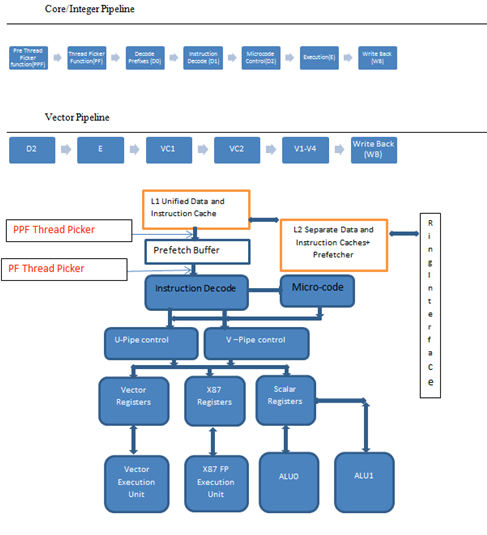
\includegraphics[width=\textwidth]{images/xeon-phi-pipeline.png}
   \caption{Pipeline de Xeon Phi, tomado de~\cite{XeonPhiBook} }
   \label{fig::xeon_phi_pipeline}
\end{figure}


El \textit{pipeline} de instrucciones tiene siete estad\'ios para las instrucciones escalares, y las
instrucciones vectoriales ocupan otras 7. Un esquema de las etapas puede verse en la figura~\ref{fig::xeon_phi_pipeline}.
El pipeline puede stallearse parcialmente si alguna de las partes sufre un stall, a diferencia de lo que ocurre en 
arquitecturas como Intel Xeon.

El pipeline tiene las fases usuales del ciclo \textit{fetch-decode-execute}), pero con algunas modificaciones.

El \textit{instruction fetch} esta dividido en dos fases para elegir el \textit{thread} por hardware a ejecutar:
\textit{Prethread picker function} (PPF) y \textit{Picker function} (PF). En la fase PPF se mueve la instrucci\'on
a uno de los 4 buffers de \textit{prefetch} que tiene cada procesador. Por cada thread hay adem\'as dos streams de
instrucciones. Si un stream es stalleado por el pipeline, se puede despachar del otro thread.

El estad\'io PF selecciona el thread a ejecutar, usando el buffer de prefetch. Cada buffer tiene espacio para dos
instrucciones (porque puede despacharse una instrucci\'on por la \textit{U-pipe} y otra por la \textit{V-pipe}). PF
funciona de manera \textit{round robin} en los buffers de prefetch. Recargar este buffer (por ejemplo cuando hay un
\textit{miss} de cache de instrucciones) toma aproximadamente 4 o 5 ciclos.

Los 4 threads de un core son multiplexados por el pipeline del mismo, de manera de que si uno de los threads esta
\textit{stalleado} se elija a otro que tenga trabajo para hacer. Se sugiere entonces el uso de al menos dos 
\textit{threads} por core para esconder latencias de memoria y de instrucciones vectoriales, y asi aumentar la performance.

Una vez que una instrucci\'on ha sido elegida para decodificarse, pasa a los estad\'ios D0 y D1, a una velocidad de
decodificaci\'on de 2 instrucciones por ciclo de \textit{clock}. De ahi son enviadas a los dos pipes para ejecutarse.
Por \'ultimo se pasa al estad\'io de \textit{writeback} (WB). No necesariamente cuando una instrucci\'on llega a esta
fase ha terminado de ejecutarse, puesto que si la operaci\'on es vectorial reci\'en termina de ejecutarse en la unidad
vectorial 5 ciclos despu\'es.

Este pipeline corto (7 etapas frente a las 20 de la arquitectura Pentium 5 en la que se basa Xeon Phi) contribuye a que
los \textit{branch predictions} tenga menor latencia, y las instrucciones escalares tengan poca latencia~\cite{IntelXeonPhiWhitePaper}.

\subsection{Estructura de cache}

Adem\'as de la unidad de vectrizaci\'on y la unidad escalar, cada procesador cuenta con 32 Kb de cache L1 y 512 Kb de cache
L2 unificada para datos y c\'odigo. Estas caches son \textit{set associative} \textit{8-way} con una linea de cache de 64 bytes. 
La cache de datos es no bloqueante, de manera que un \textit{miss} de cache de un thread en un core, 
no se produce un \textit{flush} del pipeline en los dem\'as threads.

La cache L2 mantiene su coherencia mediante el uso de un directorio distribuido de \textit{tags}. Un esquema del mismo puede
verse en la figura~\ref{fig:xeon_phi_arch_global}. El mismo esta dividido en 64 secciones y une tanto los segmentos del
directorio de tags con los cores y los controladores de memoria principal, utilizando una topolog\'ia de anillo bidireccional
con un anillo para datos, otro para direcciones y otro para confirmaciones (\textit{acknowledgements}).

Cuando ocurre un \textit{miss} de cache L2, la direcci\'on es enviada al anillo de direcciones. Si la l\'inea de cache
es de otro core, se env\'ia un request de \textit{forwarding} y los datos son enviados por el anillo de datos. Si ning\'un
core tiene esa l\'inea de cache se env\'ia un pedido a uno de los varios controladores de memoria. Cada uno de estos controladores
maneja un subconjunto del espacio de direcciones con el prop\'osito de reducir los cuellos de botella y aumentar el ancho de banda.

El protocolo de coherencia esta basado en MESI utilizando GOLS.

Cada cache L2 esta divida en dos bancos y tiene una latencia de 2 ciclos para leer 64 bytes (una l\'inea) y 1 ciclo para escribir 64 bytes.

La unidad de procesamiento vectorial lee y escribe los datos de cache con una granularidad de 512 bits, a trav\'es de un
\textit{bus} dedicado de 512 bits. Los accesos son alineados antes de ser escritos al \textit{write-commit} buffer de la
cach\'e.

La pol\'tica de cach\'e puede modificarse mediante \textit{hints} al coprocesador. Por defecto la pol\'itica del subsistema
de cach\'e es pseudo-LRU (\textit{Least Recently Used}). Antes de escribir una l\'inea de cache el procesador debe leerla a su propia
cache (pol\'tica conocida como RFO, \textit{Read For Ownership}). Dado que esto puede implicar que datos \'utiles de cache
sean removidos para dejar lugar a datos que solo se van a escribir, la arquitectura da soporte a stores \textit{stremeados},
que pasan de largo a los caches. Tambi\'en se dispone de un \textit{prefetcher} por hardware.

\subsection{Arquitectura de instrucciones}

Si bien la base del conjunto de instrucciones de la arquitectura del Xeon Phi es la P54C de Pentium (IA-32), nuevas instrucciones
se han incluido con el prop\'osito de aumentar la idoneidad del procesador para computo de alta performance. 
Estas operaciones incluyen implementaciones por \textit{hardware} de operaciones com\'unes en HPC: rec\'iproco de un valor, 
ra\'iz cuadrada, potencia y exponenciaci\'on, y operaciones m\'as relacionadas con la memoria como por ejemplo \textit{scatter and gatter} 
y stores \textit{streameados} de manera de aprovechar mejor el ancho de banda de memoria que permite la arquitectura.

El dise\~no de las instrucciones vectoriales es ternario, con dos operandos fuentes y uno destino codificados en la instrucci\'on.
Esta configuraci\'on permite una ganancia de hasta 20\% sobre la configuraci\'on usual binaria de otras arquictecturas SIMD (como
por ejemplo SSE o AVX)~\cite{BookXeonPhi}. Tambi\'en el \textit{set} de instrucciones cuenta con operaciones FMA (\textit{Fused
Multiply Add}) que utilizan los tres operandos como fuente y uno de ellos como el destino.

Una expansi\'on adicional para aprovechar los registros amplios son los registros de mascara (\textit{masked registers}).
Estos registros de 16 bits se utilizan en varias de las instrucciones vectoriales para habilitar o deshabilitar elementos
de los 16 (como m\'aximo) que tiene un registro SIMD del Xeon Phi como parte de un computo, contribuyendo a la generalidad de
las instrucciones adicionales de la arquitectura. Si un elemento del registro de m\'ascara, el valor resultado de la operaci\'on
sobre los dos elementos correspondientes de los operandos fuentes es escrito en el lugar correspondiente del operando destino.

Asi como ocurre con los 32 registros SIMD, los 8 registros de m\'ascara son
por \textit{thread}. El uso de estas m\'ascaras esta contemplado en las instrucciones, requiriendo un ciclo de clock adicional
para pasar por la \textit{Mask pipeline}. 

Las instrucciones especiales para exponenciaci\'on forman parte de la EMU (\textit{Extended Math Unit}), utilizando cuadratura
num\'erica y tablas para aproximar las funciones trascendentales por \textit{hardware}. Debido a la prevalencia en computo
cient\'ifico de estas instrucciones se busc\'o la disminuci\'on en el uso de ciclos de reloj para su c\'alculo.

La adici\'on de instrucciones sobre memoria no secuencial (\textit{scatter and gather}) resultan interesantes por su prevalencia
en HPC y porque facilitan la tarea de generaci\'on de c\'odigo vectorial en los \textit{backends} de compiladores. Tambi\'en, con
el prop\'osito de permitir un control m\'as fino de los cach\'es, los operandos en memoria para operaciones vectoriales permiten
la inclusi\'on de un atributo denominado \textit{eviction hint}. Este atributo permite determinar si los datos ser\'an o no
reusados, escribiendolos directamente a memoria si no fuese as\'i. De esta manera se evita la contaminaci\'on de cache con datos
que no ser\'an vueltos a utilizar en calculos posteriores. Como su nombre lo indica, este atributo es un consejo al coprocesador,
y este puede ignorarlo.

Por \'ultimo, tambi\'en la unidad vectorial implementa un \textit{prefetcher} por software, tanto para los caches L1 y L2. Estos
pueden combinarse con instrucciones de \textit{gather} y \textit{scatter} para disminuir los accesos a memoria y los \textit{stalls}
en retiro de instrucciones.

\subsection{Organizaci\'on de la memoria}

La memoria principal del Xeon Phi consiste de memoria RAM GDDR5 en la placa, de 8 GB. Los cores y la memoria principal son comunicados mediante el uso de 8
controladoras, conectadas mediante el anillo bidireccional, de dos canales a 5.5 Gb/s. Cada transferencia realizada es de 4 bytes. 
Esto nos da un l\'imite de ancho de banda te\'orico de 352 GB/s pero detalles de implementaci\'on de los chips limitan este valor a 200 GB/s. 

Las controladores reciben los pedidos mediante el anillo de direcciones y convierten estos en comandos para GDD5, retornando finalmente los datos en
el anillo de datos. Los dispositivos GDDR5 tienen el espacio de direcciones interlineado para distribuir mejor la carga de pedidos.

La memoria esta dividida en p\'aginas utilizando un esquema de 4 niveles, con direcciones de 64 bits~\ref{fig:xeon_phi_addressing}. El tama\~no de p\'agina soportado es de 4 Kb
o 2 Mb, siendo el esquema de 2 Mb preferido en aplicaciones de computo cient\'ifico. Como es de esperar, el Xeon Phi utiliza TLBs (\textit{Translation Lookaside
Buffers}) para disminuir la cantidad de accesos a memoria necesarios para mapear una p\'agina de memoria virtual en una f\'isica.

\subsection{Conexion Host - Coprocesador}

El Xeon Phi se conecta con su host mediante el uso de un bus PCI Express 2.0 de 16 pistas. Las transferencias pueden ser
mediante I/O programada o DMA (\textit{Direct Memory Access}). Este bus permite la transferencia no solo al host sino a
otros coprocesadores, permitiendo tener varias placas en una misma computadora. La velocidad de transferencia alcanzada
es de m\'as de 6 GB/s. DMA ocurre a velocidad de \textit{clock} del proceador, y los 8 canales de DMA pueden transferir
en paralelo. Cada transacci\'on de DMA es entre 64 y 256 bytes.

Siendo que el coprocesador dispone de su propio sistema operativo basado en Linux, lo cual incluye una implementaci\'on
de un \textit{stack} completo de TCP/IP, el bus PCI se puede utilizar para comunicar el sistema operativo del host con
el del Xeon Phi a trav\'es de protocolos como SSH (Secure SHell). Esto facilita la administraci\'on de la placa y la
transferencia de c\'odigo y datos para ejecuci\'on, y el uso del coprocesador como nodo de computaci\'on adicional en un
esquema de cluster.

La placa no tiene acceso a perif\'ericos, en particular disco duro. Para esto se puede utilizar un sistema NFS (\textit{Network
File System}) con el prop\'osito de almacenar datos en el host.

\subsection{Modos de ejecuci\'on}

Existen tres m\'etodos para ejecutar c\'odigo en el coprocesador.

\begin{enumerate}
    \item Nativo: El Xeon Phi permite correr c\'odigo directamente. Esto es gracias a la presencia de BusyBox Linux como sistema operativo,
    lo cual da soporte de sistema de archivos y entorno de ejecuci\'on. El c\'odigo puede ser enviado al Xeon Phi desde el host, y por defecto se utiliza un sistema
    de archivos montado sobre la propia RAM. 
    \item Offloading: El \textit{host} puede delegar la ejecuci\'on de ciertas porciones de c\'odigo al coprocesador. 
    Esto requiere que los datos necesarios para el c\'omputo sean copiados del \textit{host} al Xeon Phi, lo cual puede implicar que el bus puede ser un cuello de botella 
    importante (puesto que los datos de entrada, y la salida deben ser movido al Xeon Phi y traidos de vuelta al finalizar el c\'omputo).
    \item Simétrico: En este modo de ejecuci\'on se piensa al Xeon Phi y su host como dos nodos en un \textit{cluster} de c\'omputo, y al bus PCIe como una red de alta velocidad.
    Este modo es especialmente interesante si se dispone de m\'as de un Xeon Phi en un mismo host, 
    y se utiliza una interfaz de pasado de mensajes entre ellos como por ejemplo MPI (\textit{Message Passing Interface}).
\end{enumerate}

\subsection{Consumo}

El consumo energ\'etico es uno de los principales factores considerados para el dise\~no de la arquitectura MIC. La filosof\'ia
utilizada para lograr un m\'aximo equilibrio de potencia y consumo es que la aplicaci\'on dictamina al hardware como 
manejar los estados de poder que dispone. 

Existen varios estados de consumo energ\'etico: Turbo, P-states, C-states y M-states. En modo Turbo, seg\'un la cantidad de
cores ejecutando se puede incrementar la frecuencia de reloj de los mismos. La frecuencia de operaci\'on de todos los procesadores
puede modificarse usando los distintos P-states, que rigen la velocidad del clock general. Adicionalmente cada core puede estar en
distintos C-states. El procesador puede correr a su m\'axima capacidad (C0), puede no recibir el clock general pero si interrupciones
(C1), o puede estar apagado en su totalidad (C6). Existen estados similares para los controladores de memoria (M-states).

\subsection{Herramientas de desarrollo y profiling}
\subsection{Idoneidad para la tarea}

\subsection{Hardware}

La arquitectura del Xeon Phi, parte de la linea de Intel Many Core Architecture (MIC), est\'a esquematizada
en la figura~\ref{fig:xeon_phi_arch}. Cada procesador esta esquematizado en~\ref{fig:xeon_phi_core}

La base de esta arquitectura consiste entre 60 y 80 cores SMP (\textit{Symmetric Multiprocessing}), con lo cual todos
ellos comparten la misma memoria principal. Cada uno de los cores tiene un \textit{clock rate} de 1 GHz,
con una arquitectura similar al set de instrucciones de Intel IA-32. Las principales diferencias con este
conjunto de instrucciones son el soporte para direccionamiento a 64 bits y nuevas instrucciones de vectorizaci\'on.

Cada procesador tiene adem\'as soporte para 4 \textit{threads}, es decir, 4 hilos de ejecuci\'on diferentes. Adicionalmente,
cada \textit{thread} puede ejecutar dos instrucciones por ciclo de clock, mediante el uso de dos pipes: \textit{V-pipe} y \textit{U-pipe}.
Algunas instrucciones, sin embargo, solo puede ser ejecutadas en una de las dos: por ejemplo las instrucciones de vectorizaci\'on solo pueden
ser ejecutadas en la \textit{U-pipe}. Para ejecutar estas instrucciones se dispone de una unidad de vectorizaci\'on (VPU, \textit{Vector Processing Unit}).
Esta unidad cuenta 32 registros SIMD (Single Instruction Multiple Data) de 512 bits. La latencia de estas instrucciones es de 4 ciclos de clock pero permiten
operar sobre 16 valores de punto flotante de precisi\'on simple (\textit{float}) a la vez.

Adem\'as de la unidad de vectorizaci\'on y la unidad escalar, cada procesador cuenta con 32 Kb de cache L1 y 512 Kb de cache
L2. Estas caches son asociativas \textit{8-way} y su linea de cache tiene 64 bytes. La coherencia de cach\'e se mantiene
mediante un directorio distribuido de \textit{tags} (v\'ease figura~\ref{fig:xeon_phi_arch}) dividido en 64 secciones e implementado
por hardware. La memoria principal consiste de memoria RAM GDDR5 en la placa, de 8 GB con velocidad de transferencia de 5.5 GT/s en 16 canales y con transferencia de 4
bytes. Esto nos da un l\'imite de ancho de banda te\'orico de 352 GB/s pero detalles de implementaci\'on de los chips limitan este valor a 200 GB/s.

Cada procesador, puede realizar pedidos de memoria independientes sin que la memoria se convierta en un cuello
de botella importante~\cite{Fang}. Sin embargo, los 4 \textit{threads} dentro de un \textit{core} ven sus accesos a memoria serializados.

Adicionalmente los cores est\'an conectados por dos anillos bidireccionales que les permite comunicarse entre si. La velocidad de
comunicaci\'on es suficiente para considerar que todos los procesadores son sim\'etricos (es decir, cada procesador puede comunicarse con
cualquier otro con un \textit{overhead} despreciable)~\cite{Fang}.

Por \'ultimo, cada procesador tiene un \textit{in-order pipeline} de corta longitud, diferencia importante con los cores de un procesador
estandar de la arquitectura x86. El \textit{pipeline} corto implica que las operaciones escalares no tienen latencia y las vectoriales tienen baja latencia,
y el costo por \textit{branch misprediction} es bajo~\cite{IntelXeonPhiWhitePaper}. Este punto diferencia fuertemente al Xeon Phi de aceleradores de computo como las GPGPU,
que tienen alto costo en las bifuraciones de decisiones. Sin embargo, el Xeon Phi no ejecuta instrucciones de manera \textit{out-of-order}, lo cual implica que muchas
t\'ecnicas de optimizaci\'on que explotan el paralelismo a nivel instrucci\'on usuales en arquitecturas como x86-64 no son aplicables.

La otra diferencia es nuevas instrucciones de vectorizaci\'on, incompatibles con sets de vectorizaci\'on anteriores de Intel (por ejemplo AVX o SSE 4.1).
Estas operaciones incluyen implementaciones por \textit{hardware} de operaciones com\'unes en HPC: rec\'iproco de un valor, ra\'iz cuadrada, potencia y
exponenciaci\'on, y operaciones m\'as relacionadas con la memoria como por ejemplo \textit{scatter and gatter} y stores \textit{streameados} de manera de aprovechar
mejor el ancho de banda que tiene la arquitectura.

El Xeon Phi es un coprocesador, lo cual implica que necesita ser instalado sobre una computadora que sirva de \textit{host}. La comunicaci\'on con este host
ocurre a trav\'es de un bus PCI Express, no comparten ni memoria ni otros perif\'ericos como por ejemplo disco duro. Existen dos m\'etodos para acceder al Xeon~\cite{BookXeonPhi}

\begin{enumerate}
    \item Nativo: El Xeon Phi permite correr c\'odigo directamente, mediante el uso de SSH (Secure SHell). Esto es gracias a la presencia de BusyBox Linux como sistema operativo,
    lo cual da soporte de sistema de archivos y entorno de ejecuci\'on. La interfaz utiliza TCP/IP virtualizado mediante el bus PCI Express. Si bien el coprocesador no tiene acceso a \textit{storage} persistente (puesto que el sistema operativo esta montado sobre la memoria) esto puede resolverse utilizando un sistema de archivos remoto montado en la memoria del host.
    \item Offloading: El \textit{host} puede delegar la ejecuci\'on de ciertas porciones de c\'odigo al coprocesador. Esto requiere que los datos necesarios para el c\'omputo sean copiados del \textit{host} al Xeon Phi, lo cual puede implicar que el bus puede ser un cuello de botella importante (puesto que los datos de entrada, y la salida deben ser movido al Xeon Phi y traidos de vuelta al finalizar el c\'omputo).
    \item Simétrico: En este modo de ejecuci\'on se piensa al Xeon Phi y su host como dos nodos en un \textit{cluster} de c\'omputo, y al bus PCIe como una red de alta velocidad.
Este modo es especialmente interesante si se dispone de m\'as de un Xeon Phi en un mismo host, y se utiliza una interfaz de pasado de mensajes entre ellos como por ejemplo MPI (\textit{Message Passing Interface}).
\end{enumerate}

Por \'ultimo, en pos de simplificar el trabajo de adaptar una aplicaci\'on a usar el Xeon Phi, el mismo provee una unidad de monitoreo de \textit{performance} (\textit{Performance
Monitoring Tool}, PMU). Esta unidad permite la colecci\'on de informaci\'on del coprocesador, aunque no tiene soporte para ciertas caracter\'isticas com\'unes a los procesadores
de lineas m\'as est\'andar de Intel (por ejemplo: \textit{sampling} preciso de eventos por \textit{hardware}, como por ejemplo ciclos por instrucci\'on o \textit{misses} de cache).



